% Template Taken from NIPS 2012
%
% Document Properties
\documentclass[fleqn]{article}
\usepackage{nips12submit_e,times}
%
% Inserted Packages (Gregory Added)
\usepackage{enumerate}
\usepackage{subfigure}
\usepackage{appendix}
\usepackage{float}
\usepackage{amsmath}
\usepackage{algorithm, algorithmic}
\usepackage{amsfonts}%
\usepackage{amssymb}%
\usepackage{graphicx}
%
%-------------------------------------------------------------------------------
\title{Prediction of Chess Endgame using\\
Decision Tree and SVM Classifiers}

\author{
Anderson, Michael\\
CS\\ 
\texttt{andermic@eecs.oregonstate.edu} \\
\AND
Gutshall, Gregory\\
ECE\\
\texttt{gutshalg@eecs.oregonstate.edu} \\
}

\newcommand{\fix}{\marginpar{FIX}}
\newcommand{\new}{\marginpar{NEW}}

\nipsfinalcopy % Uncomment for camera-ready version

\begin{document}

\maketitle

\begin{abstract}
Traditionally, computer chess programs evaluate positions heuristically, by considering for each player factors such as the number of uncaptured pieces, king safety, central control, and number of possible moves available for both players. Chess endgame positions (positions with only a few pieces left) are often evaluated by starting from positions that are known to be won or drawn, and then working backward through a search tree. We would like to propose a third approach: formulate the problem of deciding the result of a chess endgame as a classification problem. Here we describe the application of both Decision Tree and Multi-Class SVM algorithms to a UCI dataset\cite{MichaelBain:1994} that contains 28056 King and Rook vs. King endgame positions, along with the number of moves required by white to force checkmate in each position, when possible. We show that both Decision Tree and SVM are effective algorithms, although Decision Tree somewhat outperforms SVM. We further show that reparameterizing the dataset in terms of the spatial relationships of the pieces to each other, as well as to the edges of the board, improves the performance of our classifiers.
\end{abstract}

% ***********************************************
\section{Introduction}
\label{sec:Intro}
%
\subsection[Background]{Background\textbackslash Problem Formulation}
\label{subsec:Background}
In this report, we discuss the problem of finding the number of moves required for white to beat black from an endgame position, with optimal play by both sides. In particular, we are interested in endgames where only three pieces remain on the board: a white king, a white rook, and a black king. A tried-and-true approach to this problem is to use a searching algorithm. The number of possible king and rook versus king checkmate positions is small enough that an algorithm can construct separate trees starting from all of them, and work backwards to any given king-rook king position. Using this method, along with minimax, it is then possible to determine the number of moves required by white to force checkmate with optimal play.

The issue with this approach is that search trees grow exponentially with their depth, and so minimax search requires a lot of computation time to look back more than a few moves. Here we consider another approach, that of using supervised learning to directly find the number of moves to checkmate. Instead of attempting to look forward to future positions or look back from a decisive position, we wish to look only at the current position itself. Here we test the hypothesis that simply the locations of the pieces in a given position provide enough information to determine the outcome of the game, and how far away that outcome is.
%
\begin{figure}[H]
	{\centering
		\mbox{
		\subfigure[Checkmate!]{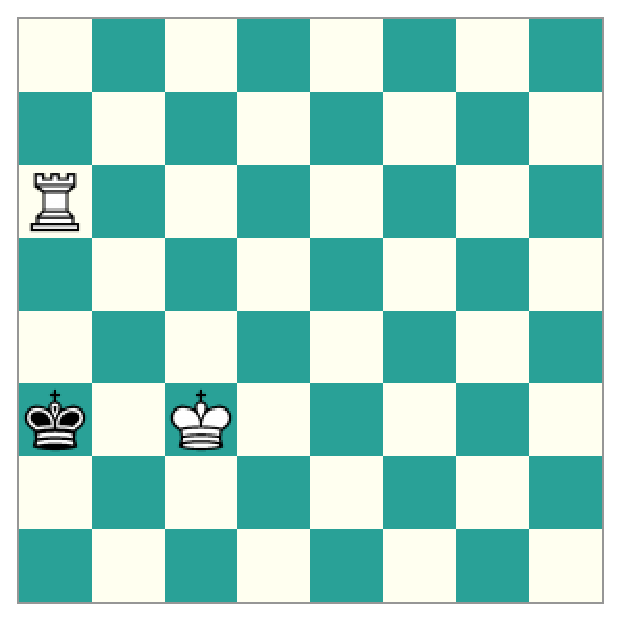
\includegraphics[trim = 0mm 0mm 0mm 0mm, clip,width=0.25\textwidth]{figs/checkmate}}\quad
		\subfigure[Free Rook]{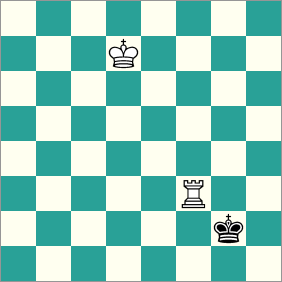
\includegraphics[trim = 0mm 0mm 0mm 0mm, clip,width=0.25\textwidth]{figs/free_rook}}\quad
		\subfigure[Free $B_k$]{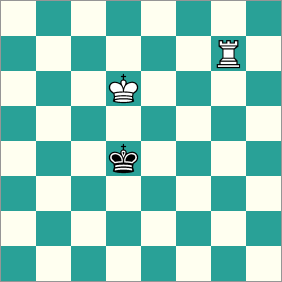
\includegraphics[trim = 0mm 0mm 0mm 0mm, clip,width=0.25\textwidth]{figs/black_king_middle}}
		}
		\caption{Example of some common Chess spatial features}
		\label{fig:ChessBoard}
	}
\end{figure}
%
In order to decide what sort of information is required to make this determination, we first need to understand the peculiarities of this problem. Figure(\ref{fig:ChessBoard}.a) shows the characteristic King-Rook King checkmating pattern; the black king is on the edge, the white king directly opposes it from two squares away, and the white rook attacks the black king. It is important to notice that the black king cannot be put into checkmate in this type of endgame without being on an edge. Figure(\ref{fig:ChessBoard}.b) shows a drawn position; black simply captures the white rook, because the white king is too far away to protect it. Figure(\ref{fig:ChessBoard}.c) shows a position with the black king in the middle of the board; here the white rook and king must work together to force the black king to the edge, and then deliver checkmate. In the given position white should move his rook 3 squares down to check the black king and force it closer to the bottom edge of the board. The black king cannot stay in the middle of the board, because the white king controls those squares. White will be able to force a repeat of this pattern, until the pattern finally reappears with the black king on the edge of the board, which will be checkmate.
%
\subsection{Outline of Report}
\label{subsec:outline}
In section(\ref{sec:Dataset}) we describe the dataset from the UCI repository used for our training and testing environment.  In section(\ref{sec:Methodology}) we will give a common framework used for testing our algorithms and we will also provide insight into the parameterizations of the original data and why we think those parameterizations will yield improved classification results.  In section(\ref{sec:Results}) we will show results heuristically drawn from simulations for the two proposed methods and discuss the problems encountered to obtain these findings.  Finally, in section(\ref{sec:Conclusions}) we will make final conclusions and possible algorithmic strategies to improve the results. 

% ***********************************************
\section{Dataset}
\label{sec:Dataset}

\subsection{Chess (King-Rook vs. King) Data Set}
\label{subsec:dataset}
Our approach was tested on an old King-Rook King dataset from the UCI website\cite{MichaelBain:1994}. This dataset contains 28056 data elements, and each element is a draw from the space of all possible King-Rook King endgame positions. The positions are uniquely described by 6 parameters: the row and column positions of each of the 3 pieces. Along with each position there is also one of 18 possible class labels $y_i \in [-1,0,1,2,3,\dots,16]$: either the position is drawn, the position is checkmate, or it will take white 1-16 moves to force checkmate with optimal play from both players.

We made a few small preprocessing modifications to this dataset to make it easier to work with. In the original dataset, rows are described using letters $(a \dots h)$, and columns using numbers $(1 \dots 8)$. We decided to make the rows numeric $(1 \dots 8)$, so that we could easily do calculations with them later. Similarly, instead of having a "draw" label and a "checkmate" label, we used the numbers $-1$ and $0$ respectively to represent these classes.
%
\subsection{Properties}
\label{subsec:Properties}
The distribution of true class labels across the dataset is not uniform, as shown by the left table:

{\centering
\begin{table}
\hspace{1cm}
\begin{tabular}{ | l | l |}
\hline
\textbf{Class} & \textbf{Count} \\ \hline
Draw & 2796 \\ \hline
Checkmate & 27 \\ \hline
1 & 78 \\ \hline
2 & 246 \\ \hline
3 & 81 \\ \hline
4 & 198 \\ \hline
5 & 471 \\ \hline
6 & 592 \\ \hline
7 & 683 \\ \hline
8 & 1433 \\ \hline
9 & 1712 \\ \hline
10 & 1985 \\ \hline
11 & 2854 \\ \hline
12 & 3597 \\ \hline
13 & 4194 \\ \hline
14 & 4553 \\ \hline
15 & 2166 \\ \hline
16 & 390 \\ \hline \hline
Total & 28056 \\ \hline
\end{tabular}
%
\hspace{2cm}
%
\begin{tabular}{| l | l |}
\hline
\textbf{Relation} & \textbf{Mutual Information} \\ \hline
I(Random, Random) & 0.003 \\ \hline
I($W_{k-row}$, Class) & 0.2903 \\ \hline
I($W_{k-column}$, Class) & 0.1653 \\ \hline
I($W_{r-row}$, Class) & 0.0462 \\ \hline
I($W_{r-column}$, Class) & 0.0501 \\ \hline
I($B_{k-row}$, Class) & 0.3145 \\ \hline
I($B_{k-column}$, Class) & 0.1851 \\ \hline \hline
$H_{total}$(Class) & 3.502 \\ \hline
\end{tabular}
\label{tab:mutalinfo}
\end{table}
}
%
This dataset has some other interesting properties, as shown by the right table of mutual information relationships between each of the parameters and the class label.

To establish a baseline, we calculated the mutual information between a vector of 28056 values drawn from $(1 \dots 8)$ and another vector of 28056 random values drawn from $(1 \dots 18)$. This told us that if there was no mutual information between a parameter and the class label, we would expect to see a mutual information of around $0.003$ from random variance. Note that the mutual information between each parameter and the class label is significantly greater than this, indicating that each one would be at least somewhat helpful in determining the value of the class label.

The most interesting thing about this table is that it shows our data is somehow skewed, and not fully representative of the population of King-Rook King endgame positions. In a representative sample, the mutual information of the row of a piece should be roughly the same as the mutual information of a column, because the four-way symmetry of the chessboard along with the four-way symmetry of the movements of king and rook indicates that each possible position has exactly one corresponding position with rows and columns transposed. Here we see that the row of the kings is more important than the column of the respective kings, which means that a classifier trained on this dataset may not generalize to the space of all possible King-Rook King endgames.

Finally, to give these mutual information numbers more meaning, we calculated the total entropy of the Class labels as $3.502$, which is an order of magnitude larger than even the best of these parameters.
%
%\subsubsection{Notation}
%\paragraph{Chess Board Positions:}
%Let the following notation describe the space of a Chess board,
%\begin{equation}
%\label{eq:StandardPositions}
%\begin{aligned}
%	\text{File} &\in \left[a,b,c,d,e,f,g,h\right]\\
%	&\in \left[1,2,3,4,5,6,7,8\right]\\
%	\text{Rank} &\in \left[1,2,3,4,5,6,7,8\right]\\
%\end{aligned}
%\end{equation}
%
%\paragraph{Game Pieces:}
%Let the three game pieces be defined as $Piece_i$, where $i = \left[1,2,3\right]$ represents the piece index,
%\begin{equation}
%\label{eq:pieces}
%\begin{aligned}
%	Piece &\in \left[W_k, W_r, B_k\right]\\
%	&W_k = \text{White King}\\
%	&W_r = \text{White Rook}\\
%	&B_k = \text{Black King}\\
%\end{aligned}
%\end{equation}
%
%\paragraph{Examples:}
%Let a example of a game be defined as $Game_j$ where $j = \left[1,2,3,\dots\right]$ is the game row index, 
%%
%\begin{equation}
%\begin{aligned}
%	Game_j &= \left[Piece_i \left\{file_j, rank_j\right\}\right]\\
%\end{aligned}
%\end{equation}
%%
%The entire set of examples is labeled as $\mathbf{X}$.
%
%\paragraph{Class Labels:}
%Class labels are defined as the remaining moves till checkmate of $B_k$.  Note, checkmate of $B_k$ is called on the $m^{\text{th}}$ move of $B_k$.
%\begin{equation}
%\begin{aligned}
%	y_j &\in \left[draw,0,1,2,3,4, \dots, m\right]\\
%	&\in \left[-1,0,1,2,3,4, \dots, m\right]
%\end{aligned}
%\end{equation}
%%
%The entire set of training class labels is labeled as $\mathbf{y}$.
%
%\subsection{Parameterization}
%\label{subsec:Parameterization}
%Discuss how we parameterized the data.
%
%Several parameter functions are used to classify or achieve an objective function, these parameter functions are labeled as $\mathbf{\Phi}\left(\mathbf{X}\right)$.
%
% ***********************************************
\section{Methodology}
\label{sec:Methodology}

\subsection{Algorithm Selection}
\label{subsec:Algorithm}
Our specific approach to this problem was to try two algorithms: Decision Tree and SVM. The selection of the Decision Tree algorithm was motivated by its successful application in a similar problem that aimed to classify a dataset of King-Rook King-Knight endgames \cite{Quinlan:83}. The selection of the SVM algorithm was motived by its reputation as a strong algorithm in many problem domains and our academic curiosity into multi-class learning with a spatial domain oriented learner.
%
\subsection{Testing\textbackslash Evaluation}
\label{subsec:Testing}
In order to evaluate our classifiers, we needed to consider how to measure error. For classification problems, error is typically evaluated as the number of mis-predicted class labels made by the classifier. However, in our problem this definition of error is somewhat uninformative, because our class labels are numeric and we want to capture how ``close'' our predicted label is to the true label. For instance, if the true class label is 14, then a prediction of 3 should constitute more error than a prediction of 15, because 3 is farther away from 14 than 15 is. Additionally, we hypothesized that it would be difficult for a classifier to distinguish between a position where forced checkmate is 14 moves away and a position where forced checkmate is 15 moves away. Taking these factors into consideration, we chose the following metric:
%
\begin{equation}
\label{eq:MeanError}
\begin{aligned}
	\mu_{error} &= \frac{1}{m} \sum_{i=1}^m |y_i - \hat{y}_i|\\
	\sigma_{error} &= \sqrt{\frac{1}{m-1} \sum_{i=1}^m |\mu_{error} - \hat{y}_i|} 
\end{aligned}
\end{equation}
%
This error metric captures average ``closeness'' of our predictions, and it does not unduly penalize incorrect predictions that are close to the true $y$. Besides our definition of error, we also needed to consider how to split up our dataset into training and testing data, since it was not neatly split as it has been in previous problems. Our approaches were slightly different for the two algorithms, and are described in their respective sections.

\subsection{Re-parameterization}
Based on our own intuition, along with previous work \cite{Quinlan:83}, we postulated that we would not be able to build strong classifiers based on the original parameterization of the data. Even though the original parameterization uniquely describes a chess position, we believed that other parameterizations would more neatly capture the information that would allow a classifier to distinguish the result of one of our endgame positions. In \cite{Quinlan:83}, instead of using the literal positions of the pieces as parameters, Quinlan uses a different set of 39 parameters that describe the spatial relationships of the pieces to one another, and the presence or absence of specific geometric configurations of the pieces. Indeed, this higher form of visual pattern recognition is more in line with how human chess players evaluate positions (along with trying to construct search trees in their heads, of course). Given this, and given what we know about the particulars of King-Rook King endgames, we were led to the following 5 parameter re-parameterizations:

\begin{enumerate}
\item L2 distance of black king to nearest corner: $\min \left\|B_k-corner_i\right\|^2$
\item L1 distance of black king to nearest edge: $\min \left\|B_k - edge_i\right\|^1$
\item L3 distance between kings: $\left\|B_k - W_k\right\|^3$
\item Draw on first move. $y_i = -1$
\item Checkmate on first move: $y_i = 0$
\end{enumerate}

We observed that our parameters give a fairly high information gain relative to the original parameters. That notwithstanding, we postulated that our parameters would outperform the original parameters because the information in our parameters was more "non-overlapping", and so that information should require fewer splits in a decision tree (for example) to unlock, as shown below,

\hspace{2.25cm}
\begin{tabular}{|l | l|}
\hline
\textbf{Relation} & \textbf{Mutual Information} \\ \hline
I($B_k$ Corner-Distance, Class) & 0.3328 \\ \hline
I($B_k$ Edge-Distance, Class) & 0.2602 \\ \hline
I($W_k$ to $B_k$ Distance L1, Class) & 0.1068 \\ \hline
I($W_k$ to $B_k$ Distance L2, Class) & 0.1488 \\ \hline
I($W_k$ to $B_k$ Distance L3, Class) & 0.1546 \\ \hline
I($W_k$ to $B_k$ Distance L4, Class) & 0.1546 \\ \hline
I($W_k$ to $B_k$ Distance L5, Class) & 0.1546 \\ \hline
I($W_k$ to $B_k$ Distance L10, Class) & 0.1546 \\ \hline
I($W_k$ to $B_k$ Distance L15, Class) & 0.1546 \\ \hline
I($W_k$ to $B_k$ Distance L18, Class) & 0.1546 \\ \hline
I($W_k$ to $B_k$ Distance L19, Class) & 0.1546 \\ \hline
I($W_k$ to $B_k$ Distance L20, Class) & 0.1541 \\ \hline
I($W_k$ to $B_k$ Distance L30, Class) & 0.1522 \\ \hline
I($W_k$ to $B_k$ Distance L50, Class) & 0.1344 \\ \hline
I($W_k$ to $B_k$ Distance L100, Class) & 0.1264 \\ \hline
I($W_k$ to $B_k$ Distance LInf, Class) & 0.1077 \\ \hline
I(Draw/No Draw, Class) & 0.4679 \\ \hline
I(Checkmate/No Checkmate, Class) & 0.0110 \\ \hline
\end{tabular}
 
% ***********************************************
\section[Results]{Simulation\textbackslash Classification Results}
\label{sec:Results}

\subsection{Results: Decision Tree}
\label{sub:resultsTrees}
For this set of experiments, we implemented a decision tree classifier that split using the information gain criterion. This included an implementation of entropy, mutual information, a trainer that builds a decision tree, and a classifier that takes a decision tree and a data element and uses the former to classify the latter. Although all of the values that any of the parameters could take were numeric, some testing showed that multi-way splits were superior to binary splits about a threshold. All of the experiments described below ran very quickly: on the order of seconds.

Our first experiment was to construct a decision tree using the original parameterization, trained on the entire dataset. Since this parameterization described each position uniquely, the decision tree had perfect accuracy in classifying our dataset. Unfortunately, this experiment created a decision tree with a whopping 27429 nodes. Since there were only 28056 elements in our dataset, this indicated that almost every split consisted of only a single data element being passed from one parent to a child, and all the rest being passed to another child. In other words, splits gave almost no information about the class label, and the tree was ridiculously overfitted to the data.

Our second experiment was to construct a decision tree using parameters from both the original parameterization, and our own 5 parameter parameterization, trained on the entire dataset. This experiment failed similarly, producing an overfitted tree with 27047 nodes.

Finally we constructed a decision tree using only the parameters in our re-parameterization, trained on the entire dataset. Note that since our parameters did not describe each position uniquely, it was not always possible for this algorithm to split until every single leaf contained only values from one class. Where leafs contained more than one class, classification of test data was done via majority vote. This experiment gave a much smaller and more reasonable model, a decision tree with 263 nodes. As a validation step, we randomly split the test data into 10 roughly equal chunks. We then performed 10 runs, in each run using a chunk as test data and the rest as training data. We originally intended to implement early stop or post-pruning to avoid overfitting issues, but this experiment demonstrated that overfitting was not a problem.

\begin{table}[htbp]
	\centering
		\begin{tabular}{ | l | c | c | c |}
  		\hline                        
  		\textbf{Method} & \textbf{$\mu$ error} & \textbf{$\sigma$ error} & \textbf{Testing Accuracy} \\ \hline
  		Decision Tree & 1.063 & 1.478 & 85.0\% \\ \hline
		\end{tabular}
	\label{table:AccuracyDT}
\end{table}
Here, testing accuracy is taken to be within a $\epsilon$-ball away from the true class label.  For this report, we used $\epsilon = 1$.  Note, since this is a multi-class problem the testing accuracy expectation for random guessing across 16 class labels is $P_y = y_i*E(y)$, where $E(y)$ is the expectation from table(\ref{tab:mutalinfo}).

\subsection{Results: Support Vector Machine (SVM)}
\label{sub:resultsSVM}

\subsubsection{Pegasos}
\label{subsub:Pegasos}
One method employed for this report was \textit{Pegasos: Primal Estimated sub\_GrAdient SOlver for SVM}\cite{Shwartz:2007}.  This is a iterative shrinkage method that alternates between stochastic gradient descent steps and projection steps.  This method does \textbf{not} improve accuracy over other SVM methods, but does drastically improve convergence time.  This speedup is achievable by approximating the sub-gradient with $k$ random samples of the training matrix and projecting $\mathbf{w}$ onto a $L_2$ ball of radius $1/\sqrt{\lambda}$, where $\lambda$ and $k$ are tunning parameters.     

To start, the Pegasos algorithm\cite{Shwartz:2007} was visually tested against the chosen parameter space to see how separable the data was (see, fig(\ref{fig:2D_Space})) and if the algorithm was working correctly.  
%
\begin{figure}[H]
	{\centering
		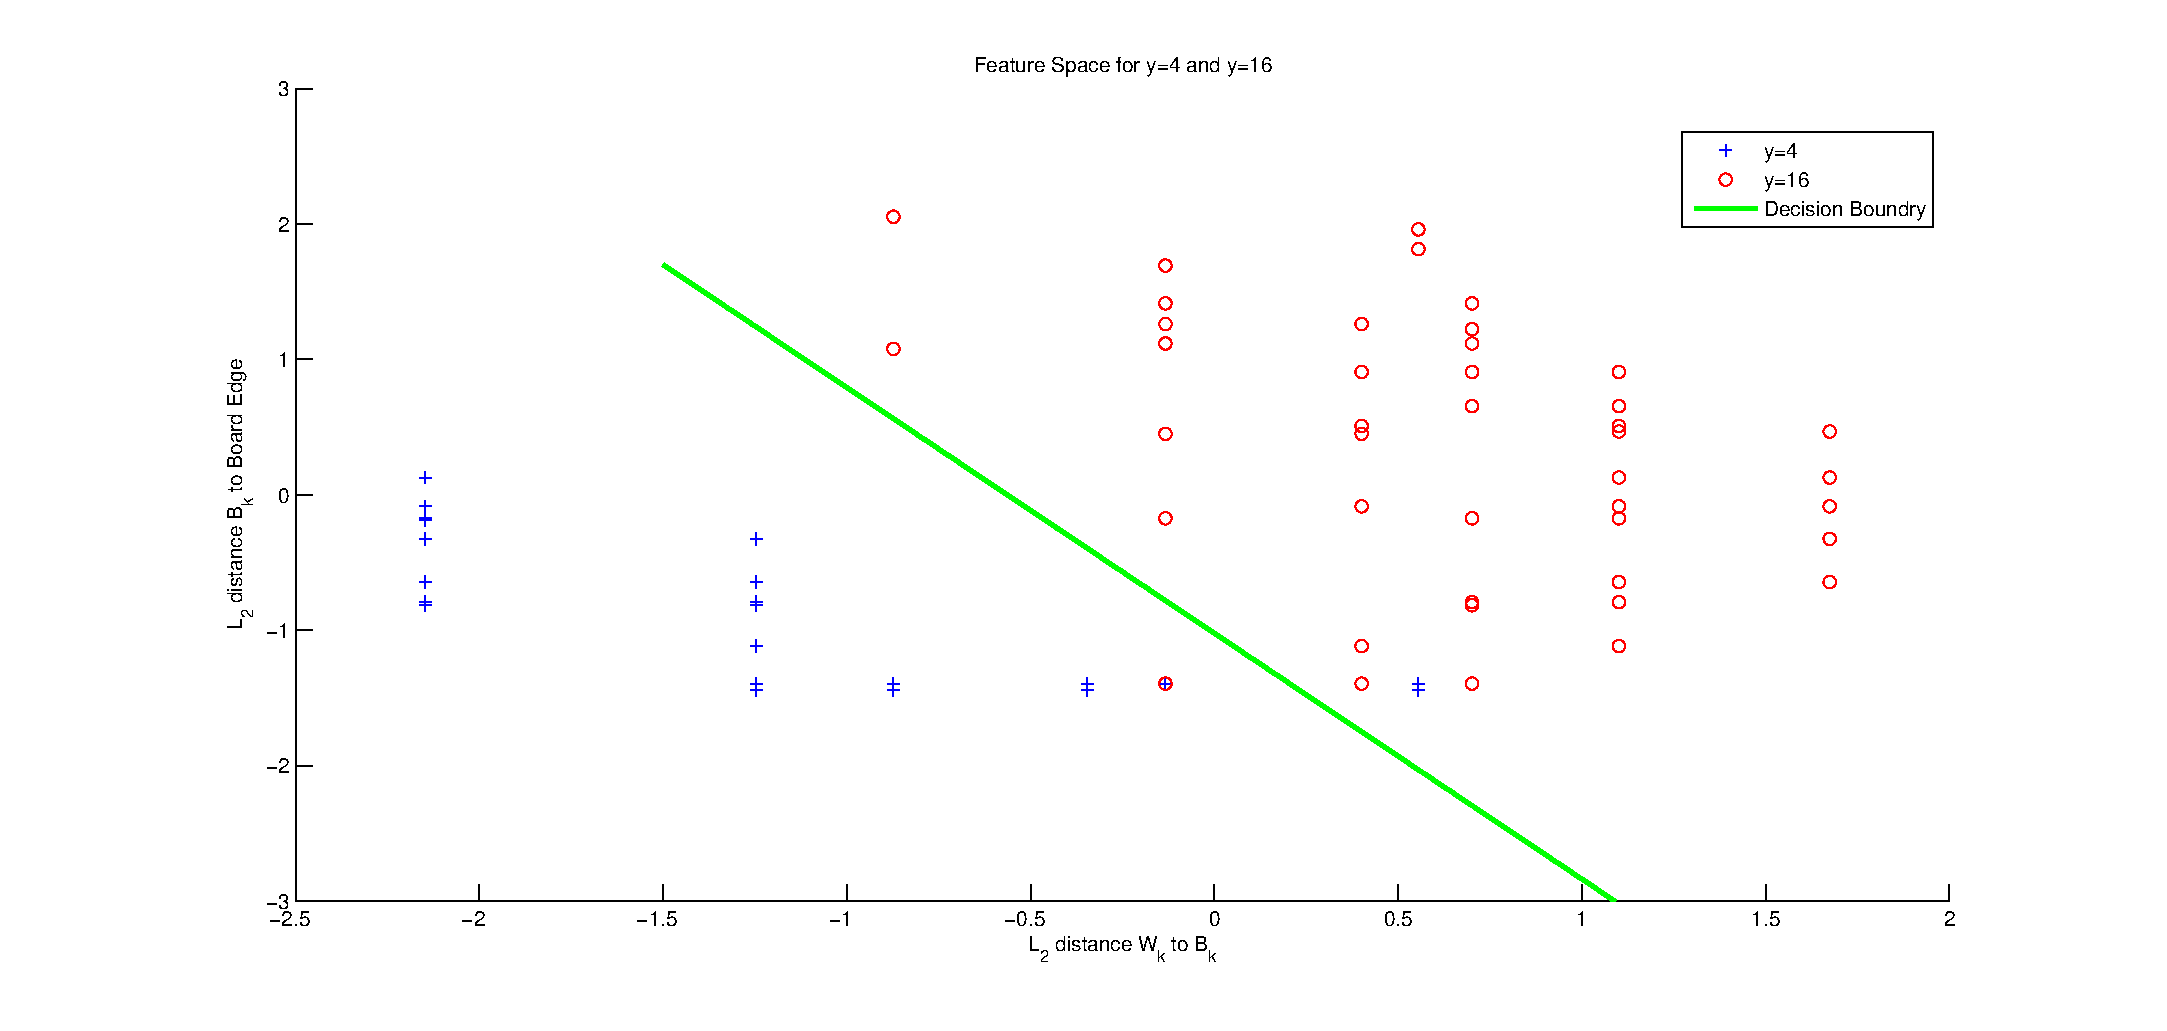
\includegraphics[trim = 10mm 8mm 10mm 0mm, clip,width=0.9\textwidth]{figs/2D_FeatureSpace}
		\caption{Feature Space Separation for two-parameters ($\left\|B_k - W_k\right\|^2$ and $\left\|B_k - corner\right\|^2$) for classes $y=4$ and $y=16$}
		\label{fig:2D_Space}
	}
\end{figure}
%
With the algorithm working, the next goal is to setup the grid-search for tunning parameters $\lambda$ and $k$.  The projection distance is controlled by $\lambda$, while the subset of training examples for the sub-gradient is controlled by $k$, i.e. $A_k \subseteq X$.  This grid-search had to be performed on each inner-class binary training problem. 
%
\begin{figure}[H]
	{\centering
		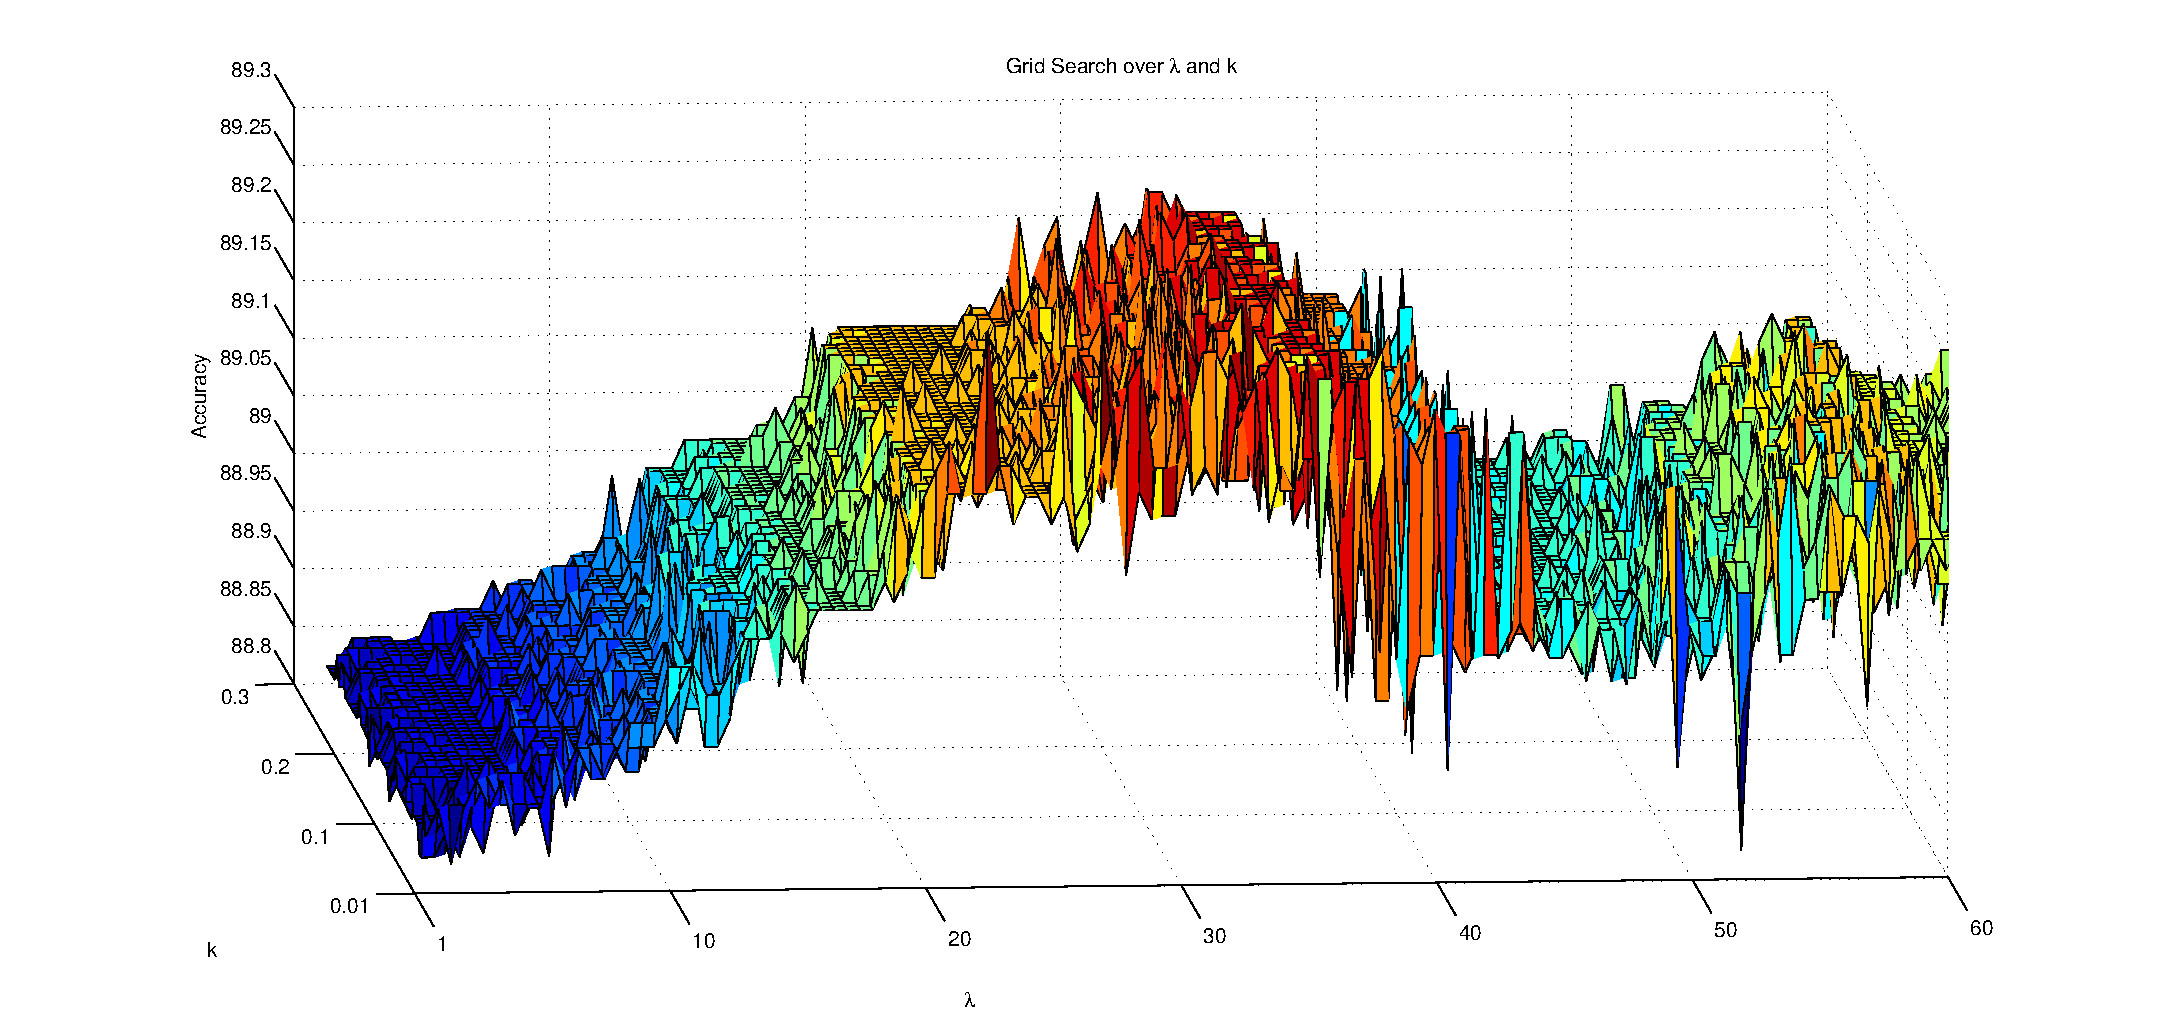
\includegraphics[trim = 10mm 8mm 10mm 0mm, clip,width=0.9\textwidth]{figs/Grid_Search}
		\caption{Grid-search over $\lambda$ and $k$ for a single binary classification instance}
		\label{fig:GridSearch}
	}
\end{figure}  

For Pegasos, we tried two methods for multi-class classification.  The first, was \textit{one-versus-the-rest}\cite{vapnik:1998}, where $K$ separate SVMs are trained, with the $k^{th}$ class assigned $+1$ and all other classes assigned to $-1$.  Then the classification is provided by $y(\mathbf{x}) = \text{max}_k y_k (\mathbf{x})$.  This provided dismal results, since the decision boundary tended to split the feature space into separate halves, giving classes $\widehat{y} = 1$ and $\widehat{y} = 16$ the farthest distance to any decision boundary. The second method, was \textit{one-versus-one}\cite{vapnik:1998}, where $K(K-1)$ separate SVMs are trained against each other.  Then the classification is provided by $y(\mathbf{x}) = \text{max}_k \rho_k y_k (\mathbf{x})$.  Where, $\rho_k$ is the number of ``votes'' for a given class $y_k$. The voting parameter $\rho_k = \sum_{i \neq I_k} (y_i = +1)$ was created by evaluating each row of the weight matrix, corresponding to a class label $\mathbf{y} \in [1,2,\dots,16]$, such that $y_i = sign(\mathbf{W}_i^T \mathbf{x} + \mathbf{b}_i)$.  

Now, it was observed from the dataset(\ref{subsec:dataset}) that the number of examples for each class was vastly different.  In this case, the SVM approximates a majority-class classifier and places the decision boundary extremely close to the minority class.
%
\begin{figure}[H]
	{\centering
		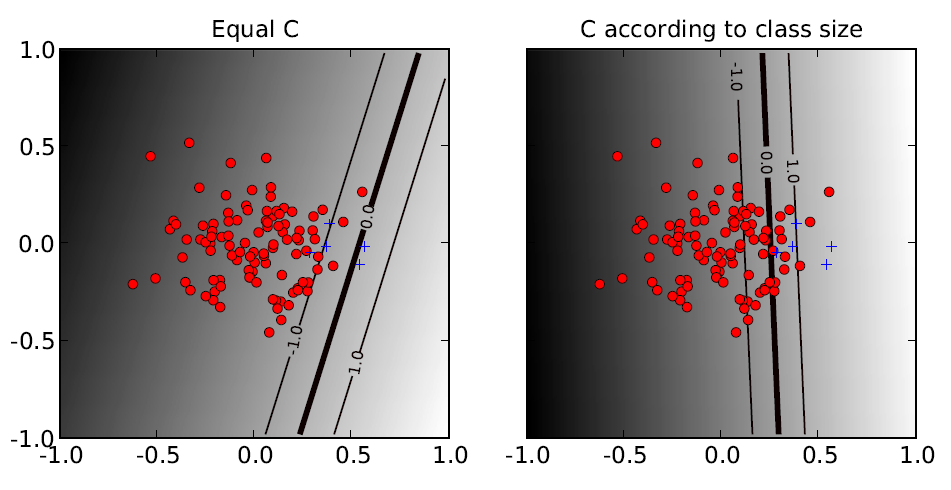
\includegraphics[trim = 2mm 2mm 2mm 2mm, clip,width=0.75\textwidth]{figs/DifferentC}
		\caption{Effect of uneven number of class examples on the decision boundary (figure from \cite{UsersGuideSVM})}
		\label{fig:Different_SVM_C_size}
	}
\end{figure}
%
To avoid majority-control, we can randomly sub-sample each class in $\mathbf{y}$ so that each minority class has the same amount of examples to train from.  In this case, I sub-sampled a set of 60 examples from each class in $\mathbf{y}$.

The final multi-class prediction was found to be,

\begin{table}[htbp]
	\centering
		\begin{tabular}{ | l | c | c | c |}
  		\hline                        
  		\textbf{Method} & \textbf{$\mu$ error} & \textbf{$\sigma$ error} & \textbf{Testing Accuracy} \\ \hline
  		Pegasos: One-v-One & 1.78 & 1.59 & 51.25\% \\ \hline
		\end{tabular}
	\label{table:AccuracyPegasos}
\end{table}

\subsubsection{LIBSVM}
\label{subsub:LIBSVM}
For Pegasos we used a linear kernel for the inner product of $\mathbf{w}^T \mathbf{x}_i$.  We can expand this to a larger dimensional space by using a polynomial kernel $K(x_i , x_j) = (\gamma x_i^T x_j + r)^d$ of various power $d$, a radial basis function (Gaussian) kernel $K(x_i , x_j) = \exp(-\gamma \left\|x_i - x_j\right\|^2)$, or a sigmoid kernel $K(x_i , x_j) = \tanh(\gamma x_i^T x_j + r)$.  The authors state that this is possible\cite{Shwartz:2007}, but I was unable to complete the coding.  So, all three non-linear kernels were attempted using the LIBSVM solver\cite{LIBSVM}.

LIBSVM comes with its own methods for handling multi-class classification.  To the end-user it is more of a \textit{``black-box''}, where $\mathbf{X}, \mathbf{y}, \text{and some [options]}$ are supplied to the function verbatim.  Again, using $\epsilon = 1$ for the testing accuracy we found the following results,

\begin{table}[htbp]
	\centering
		\begin{tabular}{ | l | c | c | c |}
  		\hline                        
  		\textbf{LIBSVM: Kernel} & \textbf{$\mu$ error} & \textbf{$\sigma$ error} & \textbf{Testing Accuracy} \\ \hline
  		 Linear & 1.29 & 1.42 & 68.28\% \\ \hline
  		 Polynomial d-2 & 1.75 & 1.93 & 59.9\% \\ \hline
  		 Polynomial d-3 & 1.32 & 1.42 & 66.7\% \\ \hline
  		 Polynomial d-4 & 1.60 & 1.71 & 61.82\% \\ \hline
  		 RBF & 1.20 & 1.37 & 70.1\% \\ \hline
  		 Sigmoid & 1.94 & 1.85 & 52.5\% \\ \hline
		\end{tabular}
	\label{table:AccuracyLIBSVM}
\end{table}

\pagebreak
% ***********************************************
\section{Conclusions}
\label{sec:Conclusions}
We see from tables(\ref{table:AccuracyDT}, \ref{table:AccuracyPegasos}, and \ref{table:AccuracyLIBSVM}) that the Decision Tree classifier outperforms SVM even with a non-linear kernel.  This is because Decision Trees are naturally advantageous for this type of problem where mutual information may be exploited to distinguish classes, where as, the SVM is a spatial classifier seeking to maximize a margin in some domain.  In addition, the Decision Tree has no major disadvantages between a binary or multi-class problem.  However, SVM is natively a binary classification method, so a multi-class voting mechanism (such as that described in \ref{subsub:Pegasos}) needs to be employed.

This multi-class problem was unique in that we were attempting to classify a numeric feature as a label.  So, we were able to use a heuristic for defining classification error (see, eq(\ref{eq:MeanError})).  For all methods, we were able to classify the correct number of positions required for checkmate to occur within an average of 2 moves. 

% ***********************************************
%\nocite{*}  %Uncomment this line to print all citations 
\bibliographystyle{IEEEbib}
\bibliography{references} 

\end{document}